\chapter{Meeting summary and activity plan examples}
\settocdepth{chapter}
\label{appendix-meeting_summaries}

\section{Introduction}

This chapter shows examples of meeting summaries produced during the lifetime of the project. Status meetings with the customer was held once a week. Every second week we had a meeting with the supervisor.

\section{Group status meeting}

\subsection*{2015-04-17 Group meeting}
Room: Skype meeting (NB!) \\
\noindent Time: 11.00 - 12.00

\subsubsection*{Agenda:}
\begin{itemize}
\setlength{\itemsep}{0cm}%
\item Standup
\item Meeting with FFI on Monday
\item Testing of WS-Nu \begin{itemize}
\setlength{\itemsep}{0cm}%
\item What’s the default behaviour when a user subscribes twice on the same topic?
\item What happens in microWSN when a user subscribes twice on the same topic?
\item If each subscription request is unique, will WSN return two messages when subscribed twice? Or will it only send one reply per endpoint. 
\item What happens if we set up a WS-Nu broker implementation where demand == true (publishers must register to publish on a topic)? The last should be tested with one WS-Nu broker running, and a publisher on a different machine (WS-Nu). It’s possible to test this with microWSN, but we don’t trust microWSN completely. Also we must work out how to change the returned server address to not be 0.0.0.0:8080 
\end{itemize}
\item Architecture 
\item Example data workflow for WSNotification Subscribe/publish request
\end{itemize}

\subsubsection*{Summary:}
\begin{itemize}
\setlength{\itemsep}{0cm}%
\item We have progress, everybody works on their respective sprint task. 
\item We need to show the log-files in the admin console. Håkon, Fredrik and Kristoffer will look into this. This will ease debugging. 
\item Starting to connect subscribers and topic in the administration console to the different services. 
\item Testing of WS-Nu as stated in the agenda. Trond and Kristoffer will look into this.
\item FFI meeting: \begin{itemize}
\setlength{\itemsep}{0cm}%
\item We must report the status on WSNotification implementation
\item Due to short time and under estimated difficulty of WSNotification, we decrease to two protocols (WSN and MQTT?)
\item Date for product delivery (ask for 15th of  may?)	
\end{itemize}
\end{itemize}

\section{Supervisor meeting}

\subsection*{2015-02-18 Meeting with supervisor}
Room: ITV-160 \\
\noindent Time: 13.00 - 14.00

\subsubsection*{Agenda:}
\begin{itemize}
\setlength{\itemsep}{0cm}%
\item Group status
\item Feedback on report
\end{itemize}

\subsubsection*{Summary:}
\begin{itemize}
\setlength{\itemsep}{0cm}%
\item Write about quality assurance in the report
\item Write about quality improvement in the report (strategy)
\item Check out your requirements, and deliberate on how they interact with your process.
\item How do we use the user stories? Why do we have them?
\item Present the process model with figures (with boxes and arrows)
\item Represent your time management with figures. Also add a Gantt diagram to visualize time available. 
\item Move the architecture after the project definition. \begin{itemize}
\setlength{\itemsep}{0cm}%
\item The same with prestudies 
\end{itemize}
\item Risk analysis: \begin{itemize}
\setlength{\itemsep}{0cm}%
\item Write about the cost of evaluating different alternatives in the Phase Gate Model
\item What’s the risk of exploring two alternatives?
\item Keep in mind the cost of prevent a risk, contra the risk of handling the risk when it arises. 
\end{itemize}
\item Check out Learned Hand and the Calculus of negligence
\item Improve the meeting agenda, so that the supervisor is more prepared 
\end{itemize}

\section{Customer meeting}

\subsection*{2015-02-19 Customer meeting using Skype}

Room: B1-120 \\
\noindent Time: 09.00 - 10.00

\subsubsection*{Agenda:}
\begin{itemize}
\setlength{\itemsep}{0cm}%
\item Project status:
\item We are still in the research phase, looking deep into Apache Apollo.
\item Successfully built it from the repository. Was quite a challenge. 
\item Currently two people are working on breaking down Apollo, while two others are looking into Scala. 
\item WS-Nu will be used as a library for WSNotification implementation
\item Started sketching up the web interface (two people are working on this)
\item Show the wireframe of the web interface
\item Ask about the report, and possibility for read through. 
\item Information about ZeroMQ
\end{itemize}

\subsubsection*{Summary:} 
It should be possible to map between different topic dialects. Also mapping between concrete-topic $\rightarrow$ simple-topic and vice versa. This is because some receivers are not capable of receiving all topic dialects. WSNotification does not support that a broker sends what kind of dialect it supports. We need to keep this problem in mind. \\

\noindent We have successfully built Apollo in IDEA, with all dependencies. Still in the research phase, so it’s quite a lot of work to do here. Two people are currently looking into Scala. By Wednesday, we will come to a conclusion on whether to use Apollo or not. \\

\noindent FFI would like detailed information about how WS-Nu is built and how we are going to use it. FFI would also prefer to get a copy of the report every time significant changes has been done. \\


\noindent WS-Nu does also have an non open-source implementation of WS-Cache (an internal NATO specification),  but we do not need to address this, keep it in mind though. \\

\clearpage

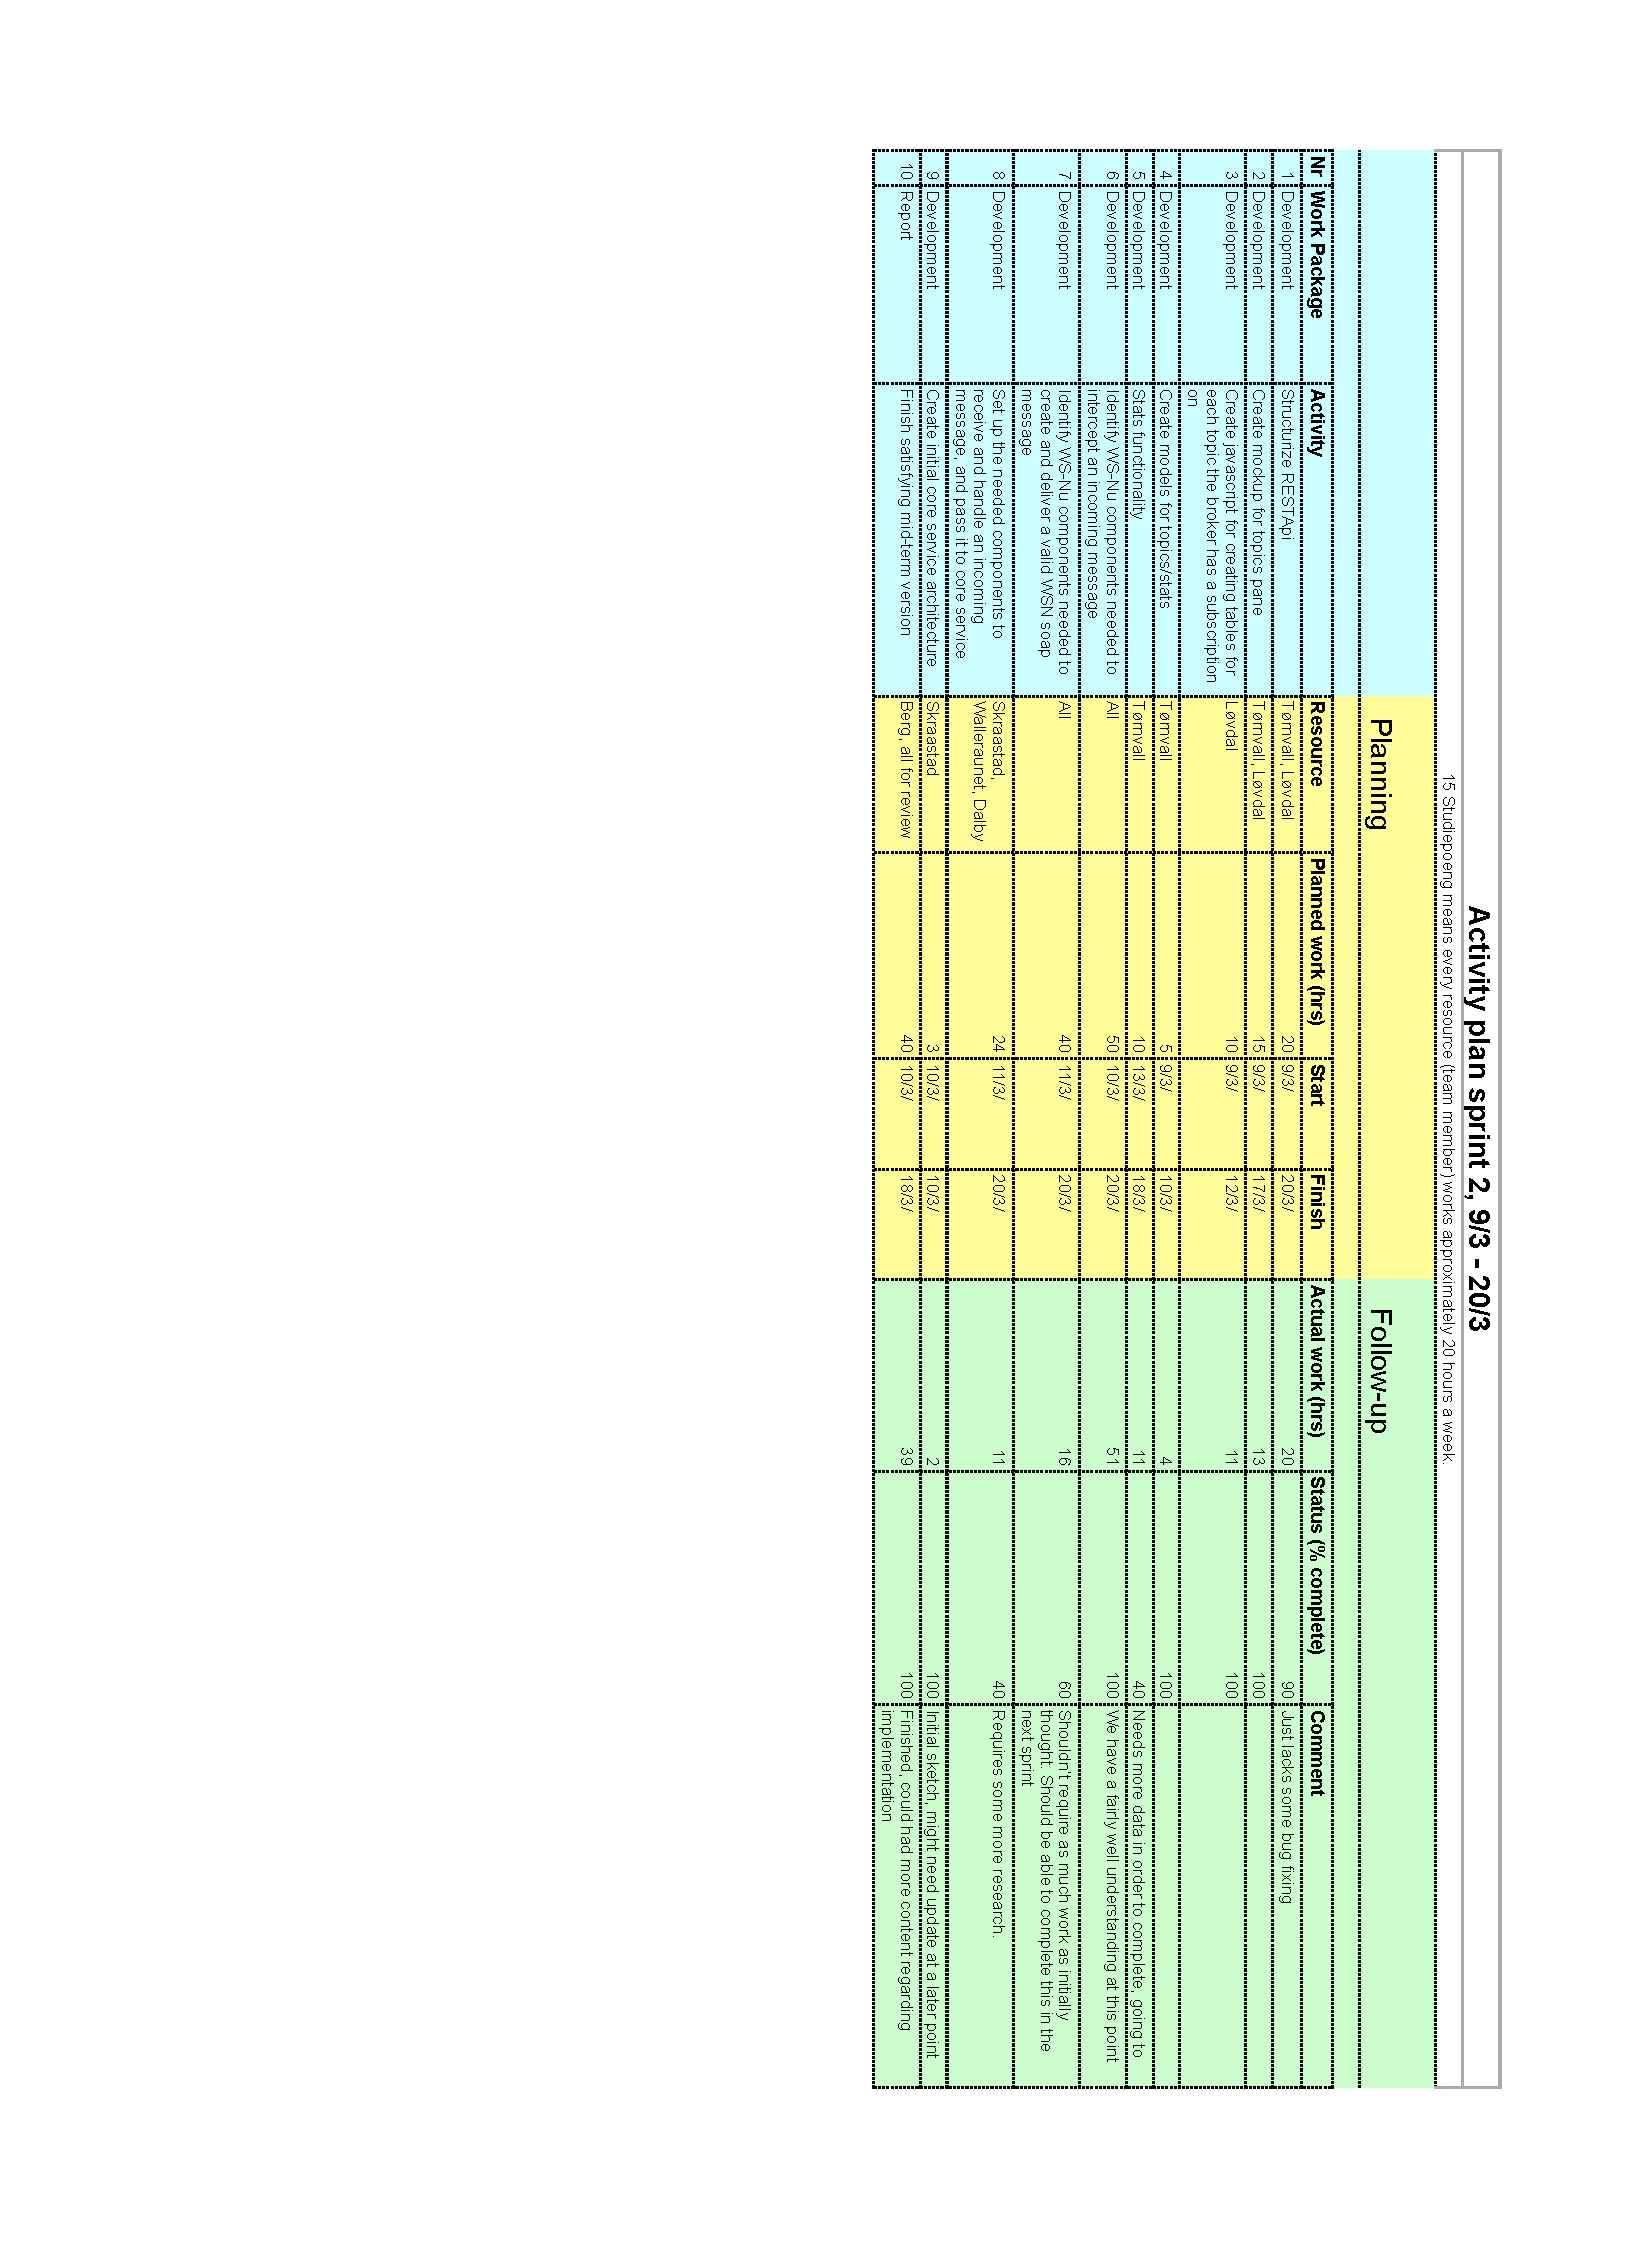
\includepdf[scale=0.7,pages=1,pagecommand=\section{Activity plan, sprint 2}]{activityplan.pdf}
\label{AppendixB:activity_plan}

\clearpage